\documentclass[11pt,letterpaper]{article}

% Packages
\usepackage[margin=1in]{geometry}
\usepackage{tikz}
\usepackage{pgfplots}
\usepackage{xcolor}
\usepackage{hyperref}
\usepackage{booktabs}
\usepackage{tabularx}
\usepackage{enumitem}
\usepackage{fancyhdr}
\usepackage{graphicx}
\usepackage{float}
\usepackage{caption}
\usepackage{subcaption}
\usepackage{amsmath}
\usepackage{fontenc}

% TikZ libraries
\usetikzlibrary{shapes.geometric, arrows.meta, positioning, fit, backgrounds, calc, decorations.markings, shadows, patterns}

% Colors - NOAA/AWS themed
\definecolor{noaablue}{HTML}{003087}
\definecolor{noaalight}{HTML}{4A90D9}
\definecolor{awsorange}{HTML}{FF9900}
\definecolor{awsdark}{HTML}{232F3E}
\definecolor{vpcgreen}{HTML}{1B660F}
\definecolor{securityred}{HTML}{CC2936}
\definecolor{neptunepurple}{HTML}{6B48FF}
\definecolor{opensearchblue}{HTML}{005EB8}
\definecolor{agentcoregold}{HTML}{D4A017}
\definecolor{fargateblue}{HTML}{2196F3}
\definecolor{lightgray}{HTML}{F5F5F5}

% Header/Footer
\pagestyle{fancy}
\fancyhf{}
\fancyhead[L]{\small\textcolor{noaablue}{NOAA/NWS/NCEP/EMC — EIB}}
\fancyhead[R]{\small\textcolor{noaablue}{MDC MCP RAG Server}}
\fancyfoot[C]{\thepage}
\renewcommand{\headrulewidth}{0.4pt}

% Hyperref setup
\hypersetup{
    colorlinks=true,
    linkcolor=noaablue,
    urlcolor=noaalight,
    citecolor=noaablue
}

\title{%
    \vspace{-1cm}
    \textcolor{noaablue}{\Large\textbf{MCP Access Architecture Proposal}}\\[0.3cm]
    \large Multi-User Scaling \& CI/CD Integration\\[0.2cm]
    \normalsize MDC MCP RAG Server — 51 AI-Powered Development Tools\\
    \normalsize for the NOAA Global Forecast System
}
\author{%
    Terry McGuinness\\
    \small Computing \& Advanced Technologies (CAT) Unit\\
    \small Environmental Modeling Center, NCEP/NWS/NOAA\\
    \small \texttt{terry.mcguinness@noaa.gov}
}
\date{April 30, 2026}

\begin{document}
\maketitle
\thispagestyle{fancy}

% ============================================================
\section{Executive Summary}
% ============================================================

The MDC MCP RAG Server provides 51 AI-powered tools for developers working on NOAA's Global Forecast System. These tools query a Neptune graph database (164,916 nodes, 2.9M relationships) and OpenSearch vector store (85,000+ documents) to provide contextual intelligence about the GFS codebase.

This document proposes a \textbf{two-phase deployment strategy}:

\begin{itemize}[leftmargin=*]
    \item \textbf{Phase 1}: Internal access for a 10-person cohort via GFE laptops with CAC-enabled VPN, using AgentCore Runtime for per-user session isolation
    \item \textbf{Phase 2}: External access for CI/CD pipelines (GitHub Actions) via FedRAMP-compliant Private API Gateway + Fargate
\end{itemize}

Both phases maintain \textbf{zero internet exposure} for the data plane and comply with NIH/NOAA security requirements.

% ============================================================
\section{System Overview}
% ============================================================

\begin{figure}[H]
\centering
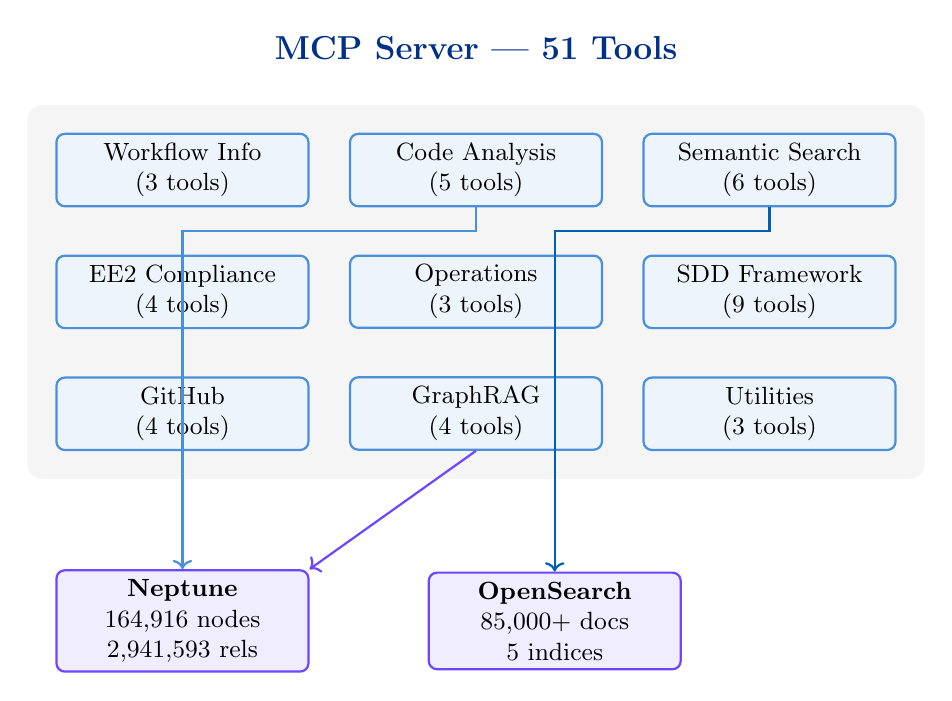
\begin{tikzpicture}[
    node distance=1.2cm,
    every node/.style={font=\small},
    box/.style={rectangle, draw, rounded corners=3pt, minimum width=3.2cm, minimum height=0.8cm, align=center, thick},
    databox/.style={box, fill=neptunepurple!10, draw=neptunepurple},
    toolbox/.style={box, fill=noaalight!10, draw=noaalight},
    countlabel/.style={font=\tiny\bfseries, text=white, fill=noaablue, rounded corners=2pt, inner sep=2pt}
]

% Tool categories
\node[toolbox] (wf) {Workflow Info\\(3 tools)};
\node[toolbox, right=0.5cm of wf] (ca) {Code Analysis\\(5 tools)};
\node[toolbox, right=0.5cm of ca] (ss) {Semantic Search\\(6 tools)};
\node[toolbox, below=0.6cm of wf] (ee) {EE2 Compliance\\(4 tools)};
\node[toolbox, below=0.6cm of ca] (op) {Operations\\(3 tools)};
\node[toolbox, below=0.6cm of ss] (sdd) {SDD Framework\\(9 tools)};
\node[toolbox, below=0.6cm of ee] (gh) {GitHub\\(4 tools)};
\node[toolbox, below=0.6cm of op] (gr) {GraphRAG\\(4 tools)};
\node[toolbox, below=0.6cm of sdd] (ut) {Utilities\\(3 tools)};

% MCP Server label
\node[above=0.8cm of ca, font=\large\bfseries, text=noaablue] (title) {MCP Server — 51 Tools};

% Data plane
\node[databox, below=1.5cm of gh] (neptune) {\textbf{Neptune}\\164,916 nodes\\2,941,593 rels};
\node[databox, right=1.5cm of neptune] (opensearch) {\textbf{OpenSearch}\\85,000+ docs\\5 indices};

% Connections
\draw[->, thick, noaalight] (ca.south) -- ++(0,-0.3) -| (neptune.north);
\draw[->, thick, opensearchblue] (ss.south) -- ++(0,-0.3) -| (opensearch.north);
\draw[->, thick, neptunepurple] (gr.south) -- (neptune.north east);

% Background
\begin{scope}[on background layer]
    \node[fit=(wf)(ca)(ss)(ee)(op)(sdd)(gh)(gr)(ut), fill=lightgray, rounded corners=5pt, inner sep=10pt] {};
\end{scope}

\end{tikzpicture}
\caption{MCP Server tool categories and backend data stores}
\label{fig:system-overview}
\end{figure}

% ============================================================
\section{Phase 1: Internal Cohort Access (10 Users)}
% ============================================================

\subsection{Architecture}

\begin{figure}[H]
\centering
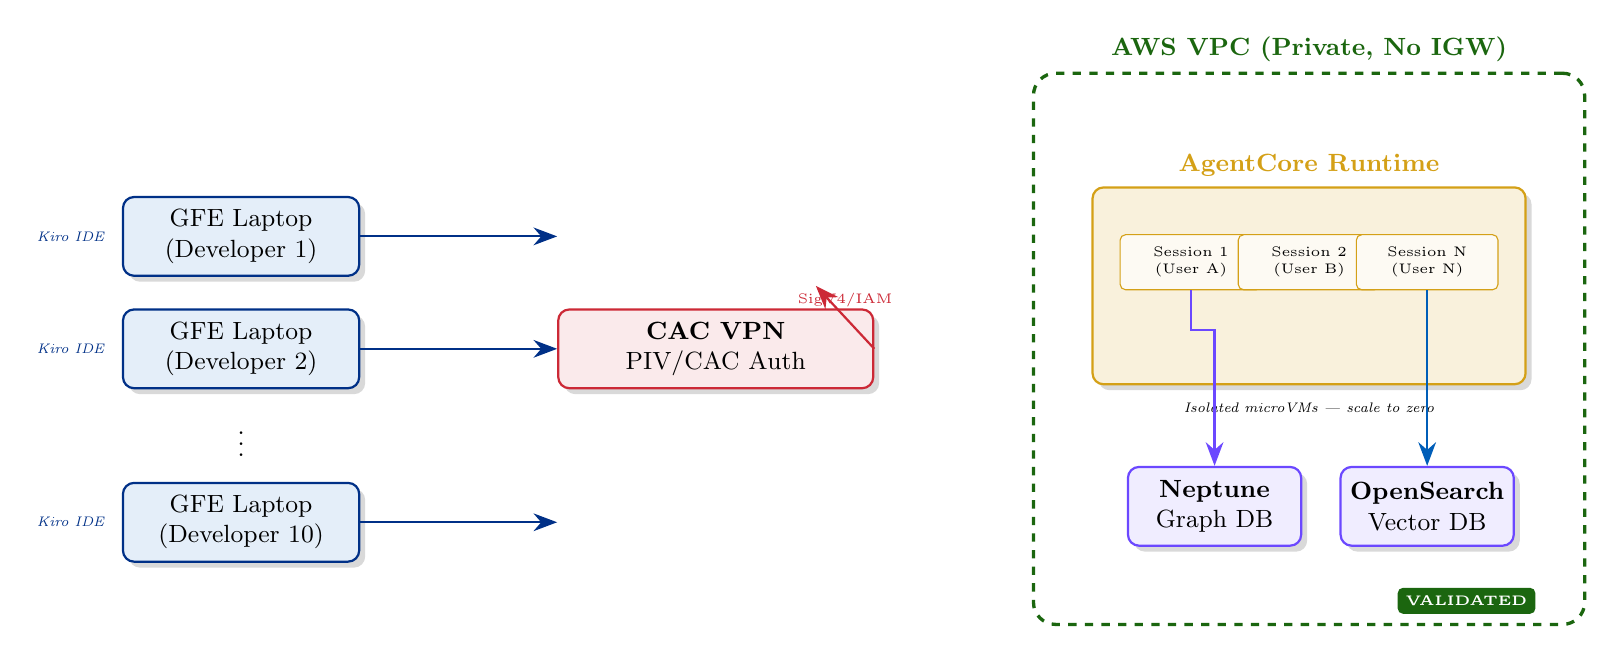
\begin{tikzpicture}[
    node distance=1.5cm,
    every node/.style={font=\small},
    box/.style={rectangle, draw, rounded corners=4pt, minimum width=3cm, minimum height=1cm, align=center, thick, drop shadow={opacity=0.3}},
    laptop/.style={box, fill=noaalight!15, draw=noaablue},
    vpn/.style={box, fill=securityred!10, draw=securityred, minimum width=4cm},
    agentcore/.style={box, fill=agentcoregold!15, draw=agentcoregold},
    microvm/.style={rectangle, draw=agentcoregold, rounded corners=2pt, minimum width=1.8cm, minimum height=0.7cm, align=center, fill=agentcoregold!5, font=\tiny},
    data/.style={box, fill=neptunepurple!10, draw=neptunepurple},
    arrow/.style={-{Stealth[length=3mm]}, thick},
    dashedarrow/.style={-{Stealth[length=3mm]}, thick, dashed}
]

% GFE Laptops
\node[laptop] (laptop1) {GFE Laptop\\(Developer 1)};
\node[laptop, below=0.4cm of laptop1] (laptop2) {GFE Laptop\\(Developer 2)};
\node[below=0.2cm of laptop2, font=\small] (dots) {$\vdots$};
\node[laptop, below=0.2cm of dots] (laptop10) {GFE Laptop\\(Developer 10)};

% Kiro label
\node[left=0.1cm of laptop1, font=\tiny\itshape, text=noaablue] {Kiro IDE};
\node[left=0.1cm of laptop2, font=\tiny\itshape, text=noaablue] {Kiro IDE};
\node[left=0.1cm of laptop10, font=\tiny\itshape, text=noaablue] {Kiro IDE};

% VPN
\node[vpn, right=2.5cm of laptop2] (vpn) {\textbf{CAC VPN}\\PIV/CAC Auth};

% VPC boundary
\node[rectangle, draw=vpcgreen, very thick, dashed, rounded corners=8pt, minimum width=7cm, minimum height=7cm, right=2cm of vpn, label={[font=\small\bfseries, text=vpcgreen]above:AWS VPC (Private, No IGW)}] (vpc) {};

% AgentCore inside VPC
\node[agentcore, minimum width=5.5cm, minimum height=2.5cm] at ([yshift=0.8cm]vpc.center) (ac) {};
\node[above=0pt of ac.north, font=\small\bfseries, text=agentcoregold] {AgentCore Runtime};

% MicroVMs
\node[microvm] at ([xshift=-1.5cm, yshift=0.3cm]ac.center) (vm1) {Session 1\\(User A)};
\node[microvm] at ([yshift=0.3cm]ac.center) (vm2) {Session 2\\(User B)};
\node[microvm] at ([xshift=1.5cm, yshift=0.3cm]ac.center) (vm3) {Session N\\(User N)};
\node[below=0.1cm of ac.south, font=\tiny\itshape] {Isolated microVMs — scale to zero};

% Data stores inside VPC
\node[data, minimum width=2.2cm] at ([xshift=-1.2cm, yshift=-2cm]vpc.center) (nep) {\textbf{Neptune}\\Graph DB};
\node[data, minimum width=2.2cm] at ([xshift=1.5cm, yshift=-2cm]vpc.center) (os) {\textbf{OpenSearch}\\Vector DB};

% Arrows
\draw[arrow, noaablue] (laptop1.east) -- (vpn.west |- laptop1.east);
\draw[arrow, noaablue] (laptop2.east) -- (vpn.west);
\draw[arrow, noaablue] (laptop10.east) -- (vpn.west |- laptop10.east);

\draw[arrow, securityred] (vpn.east) -- ([xshift=-3.5cm]ac.west) node[midway, above, font=\tiny] {SigV4/IAM};

\draw[arrow, neptunepurple] (vm1.south) -- ++(0,-0.5) -| (nep.north);
\draw[arrow, opensearchblue] (vm3.south) -- ++(0,-0.5) -| (os.north);

% Status badge
\node[fill=vpcgreen, text=white, font=\tiny\bfseries, rounded corners=2pt, inner sep=3pt] at ([xshift=2cm, yshift=-3.2cm]vpc.center) {VALIDATED \checkmark};

\end{tikzpicture}
\caption{Phase 1 — Internal cohort access via CAC VPN + AgentCore Runtime}
\label{fig:phase1}
\end{figure}

\subsection{Why AgentCore Runtime}

\begin{table}[H]
\centering
\begin{tabularx}{\textwidth}{lXX}
\toprule
\textbf{Requirement} & \textbf{AgentCore} & \textbf{Fargate} \\
\midrule
Per-user session isolation & \checkmark\ Dedicated microVM & Shared containers \\
Scale to zero (no idle cost) & \checkmark\ No sessions = \$0 & Min 1 task running \\
No capacity planning & \checkmark\ Managed fleet & Must configure scaling \\
Automatic session cleanup & \checkmark\ 15 min idle timeout & Must implement \\
Per-user observability & \checkmark\ Session-level X-Ray & Task-level only \\
\bottomrule
\end{tabularx}
\caption{AgentCore vs.\ Fargate for internal multi-user access}
\end{table}

\subsection{Authentication (Validated)}

The access pattern is already proven:
\begin{enumerate}[leftmargin=*]
    \item Developer connects GFE laptop to NOAA VPN (CAC/PIV authentication)
    \item Kiro IDE authenticates to AWS via IAM credentials (SigV4)
    \item \texttt{InvokeAgentRuntime} API call authorized by IAM policy
    \item AgentCore creates isolated microVM session for that user
    \item Session auto-terminates after 15 minutes idle
\end{enumerate}

\textbf{Status}: First user (developer lead) fully connected and operational as of April 30, 2026.

\subsection{AgentCore Runtime (Deployed)}

\begin{table}[H]
\centering
\begin{tabularx}{\textwidth}{lX}
\toprule
\textbf{Parameter} & \textbf{Value} \\
\midrule
Runtime ID & \texttt{mdc\_mcp\_rag\_server-TMXDllG2Wi} \\
Protocol & MCP (JSON-RPC at :8000/mcp) \\
Network & VPC (us-east-1a, us-east-1b) \\
Idle Timeout & 900s (15 minutes) \\
Max Lifetime & 28800s (8 hours) \\
Container & \texttt{903050880929.dkr.ecr.us-east-1.amazonaws.com/mdc-mcp-rag:agentcore} \\
Status & \textbf{READY} \\
\bottomrule
\end{tabularx}
\end{table}

% ============================================================
\section{Phase 2: CI/CD Access (GitHub Actions)}
% ============================================================

\subsection{Architecture}

\begin{figure}[H]
\centering
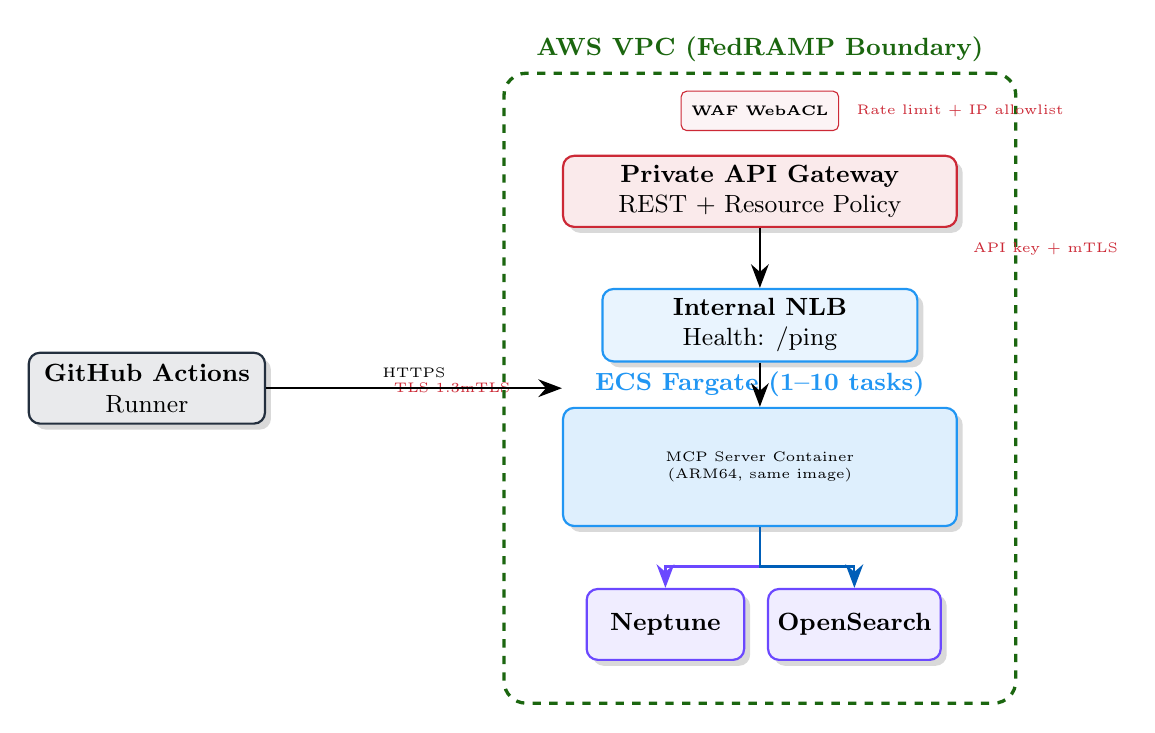
\begin{tikzpicture}[
    node distance=1.2cm,
    every node/.style={font=\small},
    box/.style={rectangle, draw, rounded corners=4pt, minimum width=3cm, minimum height=0.9cm, align=center, thick, drop shadow={opacity=0.3}},
    ghbox/.style={box, fill=awsdark!10, draw=awsdark},
    gwbox/.style={box, fill=securityred!10, draw=securityred},
    nlbbox/.style={box, fill=fargateblue!10, draw=fargateblue},
    fgbox/.style={box, fill=fargateblue!15, draw=fargateblue},
    data/.style={box, fill=neptunepurple!10, draw=neptunepurple},
    arrow/.style={-{Stealth[length=3mm]}, thick},
    waf/.style={rectangle, draw=securityred, fill=securityred!5, rounded corners=2pt, minimum width=2cm, minimum height=0.5cm, font=\tiny\bfseries}
]

% GitHub Actions
\node[ghbox] (gh) {\textbf{GitHub Actions}\\Runner};

% Internet boundary
\node[right=1.5cm of gh, font=\tiny, text=securityred] (inet) {TLS 1.3\\mTLS};

% VPC boundary
\node[rectangle, draw=vpcgreen, very thick, dashed, rounded corners=8pt, minimum width=6.5cm, minimum height=8cm, right=3cm of gh, label={[font=\small\bfseries, text=vpcgreen]above:AWS VPC (FedRAMP Boundary)}] (vpc) {};

% API Gateway
\node[gwbox, minimum width=5cm] at ([yshift=2.5cm]vpc.center) (apigw) {\textbf{Private API Gateway}\\REST + Resource Policy};

% WAF
\node[waf, above=0.3cm of apigw] (waf) {WAF WebACL};

% NLB
\node[nlbbox, minimum width=4cm] at ([yshift=0.8cm]vpc.center) (nlb) {\textbf{Internal NLB}\\Health: /ping};

% Fargate
\node[fgbox, minimum width=5cm, minimum height=1.5cm] at ([yshift=-1cm]vpc.center) (fg) {};
\node[above=0pt of fg.north, font=\small\bfseries, text=fargateblue] {ECS Fargate (1--10 tasks)};
\node[font=\tiny, align=center] at (fg.center) {MCP Server Container\\(ARM64, same image)};

% Data
\node[data, minimum width=2cm] at ([xshift=-1.2cm, yshift=-3cm]vpc.center) (nep) {\textbf{Neptune}};
\node[data, minimum width=2cm] at ([xshift=1.2cm, yshift=-3cm]vpc.center) (os) {\textbf{OpenSearch}};

% Arrows
\draw[arrow] (gh.east) -- (apigw.west |- gh.east) node[midway, above, font=\tiny] {HTTPS};
\draw[arrow] (apigw.south) -- (nlb.north);
\draw[arrow] (nlb.south) -- (fg.north);
\draw[arrow, neptunepurple] (fg.south) -- ++(0,-0.5) -| (nep.north);
\draw[arrow, opensearchblue] (fg.south) -- ++(0,-0.5) -| (os.north);

% Security annotations
\node[font=\tiny, text=securityred, right=0.1cm of waf] {Rate limit + IP allowlist};
\node[font=\tiny, text=securityred, below right=0.1cm of apigw.south east] {API key + mTLS};

\end{tikzpicture}
\caption{Phase 2 — CI/CD access via Private API Gateway + Fargate (FedRAMP-compliant)}
\label{fig:phase2}
\end{figure}

\subsection{Why Fargate for Phase 2}

\begin{table}[H]
\centering
\begin{tabularx}{\textwidth}{lXX}
\toprule
\textbf{Requirement} & \textbf{Fargate} & \textbf{AgentCore} \\
\midrule
GitHub Actions integration & \checkmark\ Standard HTTPS & Requires SDK/proxy \\
FedRAMP compliance history & \checkmark\ Well-established & Newer service \\
API Gateway + WAF & \checkmark\ Native & Not designed for this \\
Stateless CI requests & \checkmark\ Perfect fit & Session overhead \\
mTLS client certificates & \checkmark\ API GW native & Not supported \\
\bottomrule
\end{tabularx}
\caption{Fargate vs.\ AgentCore for machine-to-machine CI/CD access}
\end{table}

\subsection{FedRAMP Controls}

\begin{table}[H]
\centering
\begin{tabularx}{\textwidth}{lX}
\toprule
\textbf{Control} & \textbf{Implementation} \\
\midrule
AC-4 (Information Flow) & Private API GW, VPC endpoint, no IGW \\
AC-17 (Remote Access) & mTLS + API keys (machines); VPN + CAC (humans) \\
AU-2 (Audit Events) & CloudWatch Logs for all API GW requests \\
IA-2 (Identification) & mTLS client certs (machine); Cognito (human) \\
SC-7 (Boundary Protection) & WAF, resource policy, security groups \\
SC-8 (Transmission Confidentiality) & TLS 1.3 end-to-end \\
SC-13 (Cryptographic Protection) & KMS-encrypted at rest (Neptune, OpenSearch) \\
SI-4 (Monitoring) & X-Ray tracing, CloudWatch alarms, WAF logging \\
\bottomrule
\end{tabularx}
\caption{FedRAMP security control mapping}
\end{table}

% ============================================================
\section{Phase Comparison}
% ============================================================

\begin{figure}[H]
\centering
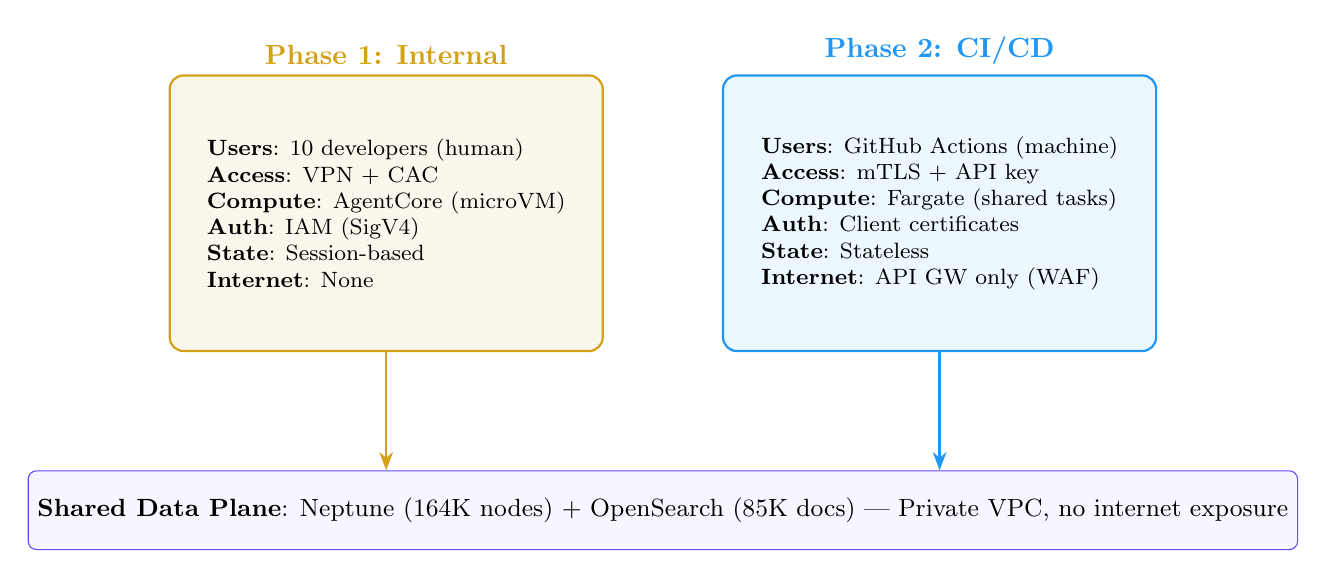
\begin{tikzpicture}[
    every node/.style={font=\small},
    phase/.style={rectangle, draw, rounded corners=5pt, minimum width=5.5cm, minimum height=3.5cm, align=center, thick},
    label/.style={font=\small\bfseries, fill=white, inner sep=2pt}
]

% Phase 1
\node[phase, fill=agentcoregold!8, draw=agentcoregold] (p1) {};
\node[above=0pt of p1.north, font=\bfseries, text=agentcoregold] {Phase 1: Internal};
\node[align=left, font=\footnotesize] at (p1.center) {
    \textbf{Users}: 10 developers (human)\\
    \textbf{Access}: VPN + CAC\\
    \textbf{Compute}: AgentCore (microVM)\\
    \textbf{Auth}: IAM (SigV4)\\
    \textbf{State}: Session-based\\
    \textbf{Internet}: None
};

% Phase 2
\node[phase, fill=fargateblue!8, draw=fargateblue, right=1.5cm of p1] (p2) {};
\node[above=0pt of p2.north, font=\bfseries, text=fargateblue] {Phase 2: CI/CD};
\node[align=left, font=\footnotesize] at (p2.center) {
    \textbf{Users}: GitHub Actions (machine)\\
    \textbf{Access}: mTLS + API key\\
    \textbf{Compute}: Fargate (shared tasks)\\
    \textbf{Auth}: Client certificates\\
    \textbf{State}: Stateless\\
    \textbf{Internet}: API GW only (WAF)
};

% Shared data plane
\node[rectangle, draw=neptunepurple, fill=neptunepurple!5, rounded corners=3pt, minimum width=12cm, minimum height=1cm, below=1.5cm of $(p1.south)!0.5!(p2.south)$] (shared) {\textbf{Shared Data Plane}: Neptune (164K nodes) + OpenSearch (85K docs) — Private VPC, no internet exposure};

% Arrows
\draw[-{Stealth}, thick, agentcoregold] (p1.south) -- (shared.north -| p1.south);
\draw[-{Stealth}, thick, fargateblue] (p2.south) -- (shared.north -| p2.south);

\end{tikzpicture}
\caption{Both phases share the same data plane with zero internet exposure}
\label{fig:comparison}
\end{figure}

% ============================================================
\section{Timeline}
% ============================================================

\begin{table}[H]
\centering
\begin{tabularx}{\textwidth}{llXl}
\toprule
\textbf{Phase} & \textbf{Milestone} & \textbf{Dependencies} & \textbf{Target} \\
\midrule
1a & AgentCore Runtime deployed & — & \textcolor{vpcgreen}{\checkmark\ Done} \\
1b & First user validated (VPN + IAM + Kiro) & — & \textcolor{vpcgreen}{\checkmark\ Done} \\
1c & 9 additional IAM users provisioned & Infra team & May 2026 \\
1d & 10-user pilot with Kiro & Onboarding & May 2026 \\
\midrule
2a & CDK stack deployment (API GW + Fargate) & Infra approval & June 2026 \\
2b & mTLS + WAF configuration & Security team & June 2026 \\
2c & GitHub Actions integration & DevOps & July 2026 \\
2d & FedRAMP documentation update & Compliance & July 2026 \\
\bottomrule
\end{tabularx}
\caption{Deployment timeline}
\end{table}

% ============================================================
\section{Cost Estimates}
% ============================================================

\begin{table}[H]
\centering
\begin{tabularx}{\textwidth}{lXr}
\toprule
\textbf{Component} & \textbf{Usage Model} & \textbf{Est.\ Monthly} \\
\midrule
\multicolumn{3}{l}{\textit{Phase 1 (AgentCore)}} \\
AgentCore compute & 10 users $\times$ 4 hrs/day $\times$ 20 days & \$40 \\
Neptune (baseline) & Already running & \$0 (existing) \\
OpenSearch (baseline) & Already running & \$0 (existing) \\
\midrule
\multicolumn{3}{l}{\textit{Phase 2 (Fargate + API GW)}} \\
API Gateway & \textasciitilde10K requests/month & \$4 \\
Fargate tasks & 1 vCPU, 2GB, auto-scale & \$30 \\
NLB & Hourly + LCU & \$16 \\
WAF & Base + per-request & \$6 \\
\midrule
\textbf{Total (both phases)} & & \textbf{\textasciitilde\$96/month} \\
\bottomrule
\end{tabularx}
\caption{Monthly cost estimates (excludes existing Neptune/OpenSearch baseline)}
\end{table}

% ============================================================
\section{Existing Assets (Ready to Deploy)}
% ============================================================

\begin{table}[H]
\centering
\begin{tabularx}{\textwidth}{lXl}
\toprule
\textbf{Asset} & \textbf{Location} & \textbf{Status} \\
\midrule
MCP Server container (ARM64) & ECR: \texttt{mdc-mcp-rag:agentcore} & \textcolor{vpcgreen}{\checkmark} \\
AgentCore Runtime & \texttt{mdc\_mcp\_rag\_server-TMXDllG2Wi} & \textcolor{vpcgreen}{\checkmark\ READY} \\
CDK Stacks (API GW + Fargate) & \texttt{infrastructure/cdk/lib/} & \textcolor{vpcgreen}{\checkmark\ 27 tests} \\
Neptune graph database & 164,916 nodes, 2.9M rels & \textcolor{vpcgreen}{\checkmark} \\
OpenSearch vector store & 85,000+ docs, 5 indices & \textcolor{vpcgreen}{\checkmark} \\
IAM execution role & \texttt{mdc-mcp-rag-ecs-task-role} & \textcolor{vpcgreen}{\checkmark} \\
Service-linked roles & All 4 AgentCore roles & \textcolor{vpcgreen}{\checkmark} \\
\bottomrule
\end{tabularx}
\end{table}

% ============================================================
\section{Next Steps}
% ============================================================

\begin{enumerate}[leftmargin=*]
    \item \textbf{Phase 1c}: Provision 9 additional IAM users with \texttt{bedrock-agentcore:InvokeAgentRuntime} permission
    \item \textbf{Phase 1d}: Onboard developers — each configures Kiro with IAM credentials (same pattern as current setup)
    \item \textbf{Phase 2a}: Deploy CDK stacks (Private API Gateway + NLB + Fargate) with infra team approval
    \item \textbf{Phase 2b}: Configure mTLS client certificates and WAF rules for GitHub Actions
\end{enumerate}

\vfill
\begin{center}
\small\textcolor{gray}{%
    Account: 903050880929 (us-east-1) | Branch: \texttt{develop\_aws}\\
    Repository: \texttt{eib-mcp-rag-server} | Wiki: \texttt{global-workflow.wiki}
}
\end{center}

\end{document}
